\documentclass{beamer}\usepackage[]{graphicx}\usepackage[]{color}
%% maxwidth is the original width if it is less than linewidth
%% otherwise use linewidth (to make sure the graphics do not exceed the margin)
\makeatletter
\def\maxwidth{ %
  \ifdim\Gin@nat@width>\linewidth
    \linewidth
  \else
    \Gin@nat@width
  \fi
}
\makeatother

\definecolor{fgcolor}{rgb}{0.345, 0.345, 0.345}
\newcommand{\hlnum}[1]{\textcolor[rgb]{0.686,0.059,0.569}{#1}}%
\newcommand{\hlstr}[1]{\textcolor[rgb]{0.192,0.494,0.8}{#1}}%
\newcommand{\hlcom}[1]{\textcolor[rgb]{0.678,0.584,0.686}{\textit{#1}}}%
\newcommand{\hlopt}[1]{\textcolor[rgb]{0,0,0}{#1}}%
\newcommand{\hlstd}[1]{\textcolor[rgb]{0.345,0.345,0.345}{#1}}%
\newcommand{\hlkwa}[1]{\textcolor[rgb]{0.161,0.373,0.58}{\textbf{#1}}}%
\newcommand{\hlkwb}[1]{\textcolor[rgb]{0.69,0.353,0.396}{#1}}%
\newcommand{\hlkwc}[1]{\textcolor[rgb]{0.333,0.667,0.333}{#1}}%
\newcommand{\hlkwd}[1]{\textcolor[rgb]{0.737,0.353,0.396}{\textbf{#1}}}%
\let\hlipl\hlkwb

\usepackage{framed}
\makeatletter
\newenvironment{kframe}{%
 \def\at@end@of@kframe{}%
 \ifinner\ifhmode%
  \def\at@end@of@kframe{\end{minipage}}%
  \begin{minipage}{\columnwidth}%
 \fi\fi%
 \def\FrameCommand##1{\hskip\@totalleftmargin \hskip-\fboxsep
 \colorbox{shadecolor}{##1}\hskip-\fboxsep
     % There is no \\@totalrightmargin, so:
     \hskip-\linewidth \hskip-\@totalleftmargin \hskip\columnwidth}%
 \MakeFramed {\advance\hsize-\width
   \@totalleftmargin\z@ \linewidth\hsize
   \@setminipage}}%
 {\par\unskip\endMakeFramed%
 \at@end@of@kframe}
\makeatother

\definecolor{shadecolor}{rgb}{.97, .97, .97}
\definecolor{messagecolor}{rgb}{0, 0, 0}
\definecolor{warningcolor}{rgb}{1, 0, 1}
\definecolor{errorcolor}{rgb}{1, 0, 0}
\newenvironment{knitrout}{}{} % an empty environment to be redefined in TeX

\usepackage{alltt}
%\usetheme{metropolis}
\usepackage[utf8]{inputenc}
\usepackage{polski}
\usepackage{amsfonts}
\usepackage{amsmath}
\usepackage{natbib}
\usepackage{graphicx}
\usepackage{array,booktabs,tabularx}
\usepackage{epstopdf}
\usepackage{colortbl, xcolor}
\usepackage{url}

\newcommand\Fontvi{\fontsize{6}{7.2}\selectfont}

\newcommand{\btVFill}{\vskip0pt plus 1filll}

\title{Komputerowe wspomaganie medycyny w bioinformatyce}
\date{}
\author{Michał Burdukiewicz}
\institute{Zakład Projektowania Systemów CAD/CAM i Komputerowego Wspomagania Medycyny}
\IfFileExists{upquote.sty}{\usepackage{upquote}}{}
\begin{document}


  

\maketitle

\begin{frame}{Plan prezentacji}

\tableofcontents

\end{frame} 

\section{Przewidywanie właściwości sekwencji biologicznych}

\begin{frame}{} 

Badania \textit{in silico} pozwalają efektywniej planować prace eksperymentalne.

Przykłady: 

\begin{itemize}
\item przewidywanie właściwości białek (np. obecność sekwencji sygnałowych, amyloidogenność),  
\item przewidywanie warunków hodowlanych mikroorganizmów.
\end{itemize}

\end{frame}   
  
\begin{frame}{Cel} 

Opracowanie metodologii analizy sekwencji biologicznych opierającej się na zrozumiałych dla człowieka regułach decyzyjnych. 

\end{frame}   

\section{n-gramy i uproszczone alfabety}

\begin{frame}
n-gramy (k-tuple, k-mery):
\begin{itemize}
\item podsekwencje (ciągłe lub z przerwami) $n$ reszt aminokwasowych lub nukleotydowych,
\item bardziej informatywne niż pojedyncze reszty.
\end{itemize}
\end{frame}  

\begin{frame}



Peptyd I: \textcolor{red}{\texttt{FKVWPDHGSG}}

Peptyd II: \textcolor{blue}{\texttt{YMCIYRAQTN}}

\medskip

Przykłady n-gramów uzyskanych z peptydów I i II:

\begin{enumerate}
    \item 1-gramy: \textcolor{red}{\texttt{F}}, \textcolor{blue}{\texttt{Y}}, \textcolor{red}{\texttt{K}}, \textcolor{blue}{\texttt{M}},
    \item 2-gramy: \textcolor{red}{\texttt{FK}}, \textcolor{blue}{\texttt{YM}}, \textcolor{red}{\texttt{KV}}, \textcolor{blue}{\texttt{MC}},
    \item 2-gramy (nieciągłe): \textcolor{red}{\texttt{F-V}}, \textcolor{blue}{\texttt{Y-C}}, \textcolor{red}{\texttt{K-W}}, \textcolor{blue}{\texttt{M-I}},
    \item 3-gramy (nieciągłe): \textcolor{red}{\texttt{F--WP}}, \textcolor{blue}{\texttt{Y--IY}}, \textcolor{red}{\texttt{K--PD}}, \textcolor{blue}{\texttt{M--YR}}.
\end{enumerate}

\end{frame}

\begin{frame}{Uproszczone alfabety}
Uproszczone alfabety:
\begin{itemize}
\item aminokwasy są grupowane w większe zbiory na podstawie 
określonych kryteriów,
\item łatwiejsze przewidywanie struktur~\citep{murphy_simplified_2000},
\item tworzenie bardziej uogólnionych modeli.
\end{itemize}
\end{frame}


\begin{frame}{Uproszczone alfabety}
Poniższe peptydy wydają się być całkowicie różne pod względem składu aminokwasowego.

Peptyd I: 

\texttt{FKVWPDHGSG}

\medskip

Peptyd II: 

\texttt{YMCIYRAQTN}

\end{frame}  


\begin{frame}

\includegraphics[width=\maxwidth]{figure/unnamed-chunk-2-1} 


\end{frame}  

\begin{frame}
\begin{table}
\begin{tabular}{cl}
\toprule
Grupa & Aminokwasy \\ 
\midrule
 \textcolor{green}{1} & \textcolor{green}{C, I, L, K, M, F, P, W, Y, V} \\ 
 \textcolor{orange}{2} & \textcolor{orange}{A, D, E, G, H, N, Q, R, S, T} \\ 
\bottomrule
\end{tabular}
\end{table}

\begin{columns}
\begin{column}{0.15\textwidth}
 
Peptyd I: 

Peptyd II: 

\end{column}
\begin{column}{0.1\textwidth}

\texttt{\textcolor{green}{FKVWP}}\texttt{\textcolor{orange}{DHGSG}} 

\texttt{\textcolor{green}{YMCIY}}\texttt{\textcolor{orange}{RAQTN}} 

\end{column}
\begin{column}{0.02\textwidth}  %%<--- here

\textrightarrow

\textrightarrow
\end{column}
\begin{column}{0.1\textwidth}  %%<--- here

\texttt{\textcolor{green}{11111}}\texttt{\textcolor{orange}{22222}}

\texttt{\textcolor{green}{11111}}\texttt{\textcolor{orange}{22222}}
\end{column}
\end{columns}
\end{frame}  



\subsection{Przewidywanie amyloidów}

\begin{frame}{Białka amyloidowe}

Agregaty białek amyloidowe występują w tkankach osób cierpiących na zaburzenia 
neurodegeneracyjne, takie jak choroba Alzheimera i Parkinsona, a także wiele innych 
schorzeń.

\begin{figure} 
\includegraphics[width=0.61\textwidth]{static_figure/amyloid_aggregates.jpg}
\end{figure}

\footnotesize
Agregaty amyloidowe (czerwone) wokół neuronów (zielone). Strittmatter Laboratory, Yale University.

\end{frame}  

  
\begin{frame}{Białka amyloidowe}

Za agregację białek amyloidogennych odpowiedzialne są sekwencje peptydowe o właściwościach amyloidogennych (hot spots):

\begin{itemize}
\item krótkie (6-15 aminokwasów),
\item bardzo zmienny, zazwyczaj hydrofobowy skład aminokwasowy,
\item tworzą unikalne $\beta$-struktury.
\end{itemize}

\begin{figure} 
\includegraphics[width=0.9\textwidth]{static_figure/zipper_structure.jpg}
\end{figure}

\footnotesize\citet{sawaya_atomic_2007}
\end{frame}


\begin{frame}{AmyloGram}
AmyloGram: oparte na analizie n-gramowej narzędzie do przewidywania amyloidów~\citep{burdukiewicz_prediction_2016, BurdukiewiczAmyloidogenicmotifsrevealed2017a}.
\end{frame}


\begin{frame}

\vspace{2cm}

\begin{figure} 
\includegraphics[width=0.95\textwidth]{static_figure/ngram1.eps}
\end{figure}

\btVFill

\tiny{Burdukiewicz, M., Sobczyk, P., Rödiger, S., Duda-Madej, A., Mackiewicz, P., and Kotulska, M. (2017). Amyloidogenic motifs revealed by n-gram analysis. Scientific Reports 7, 12961}

  \end{frame}

\begin{frame}{Walidacja krzyżowa}
\begin{knitrout}
\definecolor{shadecolor}{rgb}{0.969, 0.969, 0.969}\color{fgcolor}

{\centering \includegraphics[width=\maxwidth]{figure/unnamed-chunk-3-1} 

}



\end{knitrout}
\btVFill

\tiny{Burdukiewicz, M., Sobczyk, P., Rödiger, S., Duda-Madej, A., Mackiewicz, P., and Kotulska, M. (2017). Amyloidogenic motifs revealed by n-gram analysis. Scientific Reports 7, 12961}
\end{frame}

\begin{frame}{Najlepszy uproszczony alfabet}

   \begin{table}[ht]
\centering
\begin{tabular}{rl}
  \toprule
Grupa & Aminokwasy \\ 
  \midrule
  1 & G \\ 
   \rowcolor[gray]{0.85}  2 & K, P, R \\ 
    3 & I, L, V \\ 
   \rowcolor[gray]{0.85}  4 & F, W, Y \\ 
    5 & A, C, H, M \\ 
   \rowcolor[gray]{0.85}  6 & D, E, N, Q, S, T \\ 
   \bottomrule
\end{tabular}
\end{table}
   \btVFill

\tiny{Burdukiewicz, M., Sobczyk, P., Rödiger, S., Duda-Madej, A., Mackiewicz, P., and Kotulska, M. (2017). Amyloidogenic motifs revealed by n-gram analysis. Scientific Reports 7, 12961}
   \end{frame}

     \begin{frame}{Najlepszy uproszczony alfabet}
   \begin{table}[ht]
\centering
\begin{tabular}{rl}
  \toprule
Grupa & Aminokwasy \\ 
  \midrule
  1 & G \\ 
   \rowcolor[gray]{0.85}  2 & K, P, R \\ 
   \rowcolor{blue!20} 3 & I, L, V \\ 
   \rowcolor{blue!20}  4 & F, W, Y \\ 
    5 & A, C, H, M \\ 
   \rowcolor[gray]{0.85}  6 & D, E, N, Q, S, T \\ 
   \bottomrule
\end{tabular}
\end{table}
   
Grupy 3 i 4 - aminokwasy hydrofobowe.  
\btVFill

\tiny{Burdukiewicz, M., Sobczyk, P., Rödiger, S., Duda-Madej, A., Mackiewicz, P., and Kotulska, M. (2017). Amyloidogenic motifs revealed by n-gram analysis. Scientific Reports 7, 12961}
   \end{frame}
  
  
     \begin{frame}{Najlepszy uproszczony alfabet}
   \begin{table}[ht]
\centering
\begin{tabular}{rl}
  \toprule
Grupa & Aminokwasy \\ 
  \midrule
  1 & G \\ 
   \rowcolor{red!20}  2 & K, P, R \\ 
    3 & I, L, V \\ 
   \rowcolor[gray]{0.85}  4 & F, W, Y \\ 
    5 & A, C, H, M \\ 
   \rowcolor[gray]{0.85}  6 & D, E, N, Q, S, T \\ 
   \bottomrule
\end{tabular}
\end{table}
   
Grupa 2 - reszty aminokwasowe zakłócające $\beta$-struktury.  
   \btVFill

\tiny{Burdukiewicz, M., Sobczyk, P., Rödiger, S., Duda-Madej, A., Mackiewicz, P., and Kotulska, M. (2017). Amyloidogenic motifs revealed by n-gram analysis. Scientific Reports 7, 12961}
   \end{frame}  
   

\begin{frame}{}
Czy informatywne n-gramy znalezione przez QuiPT są związane z amyloidogennością?

Spośród 65 najbardziej informatywnych n-gramów, 15 (23\%) jest również obecnych w motywach aminokwasowych znalezionych ekperymentalnie~\citep{paz_sequence_2004}.

\tiny{Burdukiewicz, M., Sobczyk, P., Rödiger, S., Duda-Madej, A., Mackiewicz, P., and Kotulska, M. (2017). Amyloidogenic motifs revealed by n-gram analysis. Scientific Reports 7, 12961}
\end{frame}


\begin{frame}{Porównanie z innymi narzędziami}

\begin{table}[ht]
\centering

\begin{tabular}{ccccc}
  \toprule
Program & AUC & MCC \\ 
  \midrule
AmyloGram & \textbf{0.8972} & \textbf{0.6307} \\ 
  \rowcolor{white}PASTA 2.0 \citep{walsh_pasta_2014} & 0.8550 & 0.4291  \\ 
   FoldAmyloid \citep{garbuzynskiy_foldamyloid:_2010} & 0.7351 & 0.4526  \\ 
  \rowcolor{white}APPNN \citep{familia_prediction_2015} & 0.8343 & 0.5823  \\ 
   \bottomrule
\end{tabular}
\end{table}

Klasyfikator wytrenowany z wykorzystaniem najlepszego uproszczonego alfabetu, AmyloGram, został porównany z innymi narzędziami do przewidywania amyloidów z użyciem zewnętrznego zbioru danych \textit{pep424}.
\btVFill
\tiny{Burdukiewicz, M., Sobczyk, P., Rödiger, S., Duda-Madej, A., Mackiewicz, P., and Kotulska, M. (2017). Amyloidogenic motifs revealed by n-gram analysis. Scientific Reports 7, 12961}


\end{frame}



\begin{frame}{Walidacja eksperymentalna}
\begin{figure} 
\includegraphics[width=0.95\textwidth]{static_figure/FalsePositives.eps}
\end{figure}
\end{frame}

\begin{frame}{Walidacja eksperymentalna}
\begin{figure} 
\includegraphics[width=0.95\textwidth]{static_figure/ExperimentalValidation.eps}
\end{figure}
\end{frame}

\begin{frame}{Nowe białko amyloidowe}

\includegraphics[width=0.75\textwidth]{static_figure/line.jpg}

Nowy amyloid funkcjonalny produkowany przez Methanospirillum sp. \citep{10.3389/fmicb.2018.02729} został wybrany do analiz \textit{in vitro} dzięki wskazaniom AmyloGramu.

\end{frame}

\subsection{Przewidywanie peptydów sygnałowych}

\begin{frame}{Peptydy sygnałowe}

\begin{figure} 
\includegraphics[width=0.75\textwidth]{static_figure/SP.eps}
\end{figure}

Peptydy sygnałowe:
        \begin{itemize}[<+->]
          \item krótkie (20-30 reszt) N-końcowe fragmenty białek tworzące $\alpha$-helisy,
            \item kierują białka do układu wewnątrzbłonowego a następne do sekrecji lub kompartymentów wewnątrzkomórkowch.
        \end{itemize}
\end{frame}


  
\begin{frame}{Peptydy sygnałowe}

\begin{figure} 
\includegraphics[width=0.75\textwidth]{static_figure/SP.eps}
\end{figure}

Peptydy sygnałowe są bardzo zmienne, ale zawsze zawierają trzy charakterystyczne domeny~\citep{hegde_surprising_2006}:
\begin{itemize}
        \item n-region: 5-8 dodatnio naładowanych reszt aminokwasowych~\citep{nielsen_prediction_1998},
        \item h-region: bardzo hydrofobowe reszty~\citep{nielsen_prediction_1998},
        \item c-region: kilka (3-5) polarnych reszt.
\end{itemize}

\end{frame}


%Peptydy sygnałowe rozpoczynają się naładowanym dodatnio n-regionem, po którym występuje hydrofobowy h-region i c-region zakończony miejscem cięcia rozpoznawanym przez peptydazę sygnałową. 

  
\begin{frame}{Peptydy sygnałowe}  
Skład aminokwasowy peptydów sygnałowych u \textit{Plasmodium} sp. (do których należy m. in. zarodziec malarii) jest inny od składu peptydów sygnałowych innych eukariontów. Dlatego też narzędzia do przewidywania peptydów sygnałowych źle radzą sobie z przewidywaniem peptydów sygnałowych u \textit{Plasmodium} sp.


\includegraphics[width=\maxwidth]{figure/unnamed-chunk-5-1} 


PCA częstości aminokwasów.
\end{frame}  

\begin{frame}{signalHsmm}

signalHsmm \citep{BurdukiewiczPredictionSignalPeptides2018}: zastosowanie ukrytych modeli semi-Markowa i uproszczonych alfabetów aminokwasowych w celu przewidywania peptydów sygnałowych w białkach \textit{Plasmodium} sp.

\begin{figure} 
\includegraphics[width=0.75\textwidth]{static_figure/HSMMs.eps}
\end{figure}

\end{frame}

\begin{frame}{Porównanie z innymi predyktorami}
signalHsmm efektywnie uczy się rozpoznawać peptydy sygnałowe na bardzo małych zbiorach danych.

Przewidywania signalHsmm są na tyle uniersalne, że pozwalają również przewiywać nietypowe peptydy sygnałowe spotykane w białkach \textit{Plasmodium} sp.

W celu porównania się z innymi klasyfikatorami, powstały dwie iteracje signalHsmm: signalHsmm-2010, oparty na peptydach sygnałowych użytych do uczenia signalP 4.1~citep{petersen_signalp_2011} oraz signalHsmm-1987, oparty na danych dostępnych w 1987, kiedy opublikowano pierwsze narzędzie do przewidywania peptydów sygnałowych.

\btVFill

\tiny Burdukiewicz, M., Sobczyk, P., Chilimoniuk, J., Gagat, P., and Mackiewicz, P. (2018). Prediction of Signal Peptides in Proteins from Malaria Parasites. International Journal of Molecular Sciences 19, 3709.

\end{frame}

\begin{frame}{Porównanie z innymi predyktorami}

\begin{table}[H]
\centering
\small
\begin{tabular}{rllll}
  \toprule
Algorytm & Czułość & Swoistość & MCC & AUC \\ 
  \midrule
signalP 4.1 (no tm) & 0.8235 & 
0.9100 & 0.6872 & 
0.8667 \\ 
   \rowcolor[gray]{0.85}signalP 4.1 (tm) 
& 0.6471 & 
0.9431 & 0.6196 & 0.7951 \\ 
  signalP 3.0 (NN) & 0.8824 
& 0.9052 & 0.7220 & 
0.8938 \\ 
   \rowcolor[gray]{0.85}signalP 3.0 (HMM) 
 & 0.6275 & 
0.9194 & 0.5553 & 0.7734 \\ 
  PrediSi & 0.3333 & \textbf{0.9573} 
& 0.3849 & 0.6453 
\\ 
   \rowcolor[gray]{0.85}Philius 
& 0.6078 & 
0.9336 & 0.5684 & 0.7707 \\ 
  Phobius & 0.6471 & 0.9289 & 
0.5895 & 0.7880 \\ 
   \rowcolor[gray]{0.85}signalHsmm-2010 & 0.9804 & 0.8720 & 0.7409 & 0.9262 \\ 
  signalHsmm-2010 (ident. 50\%) & \textbf{1.0000} & 0.8768 & \textbf{0.7621} & 
\textbf{0.9384} \\ 
   \rowcolor[gray]{0.85}signalHsmm-2010 (pełny alfabet) & 0.8431 & 0.9005 & 0.6853 & 
0.8718 \\ 
  signalHsmm-1987 & 0.9216 & 0.8910 & 0.7271 & 0.9063 \\ 
   \rowcolor[gray]{0.85}signalHsmm-1987 (ident. 50\%) & 0.9412 & 0.8768 & 0.7194 
& 
0.9090 \\ 
  signalHsmm-1987 (pełny alfabet) & 0.7647 & 0.9052 & 0.6350 & 0.8350 \\ 
   \bottomrule
\end{tabular}
\end{table}

\tiny Burdukiewicz, M., Sobczyk, P., Chilimoniuk, J., Gagat, P., and Mackiewicz, P. (2018). Prediction of Signal Peptides in Proteins from Malaria Parasites. International Journal of Molecular Sciences 19, 3709.


\end{frame}

\section{Analiza danych z eksperymentów PCR}

\begin{frame}{PCR}

PCR (Polymerase Chain Reaction, reakcja łańcuchowa polimerazy): metoda amplifikowania DNA.

\begin{figure} 
\includegraphics[width=0.38\textwidth]{static_figure/addgene.png}
\end{figure}

\tiny Żródło: Addgene.

\end{frame}

\begin{frame}{PCR}

PCR jest powszechnie stosowany w diagnostyce medycznej, kryminalistyce i biologii molekularnej. 

\end{frame}

\begin{frame}{PCR w R}
\begin{figure} 
\includegraphics[width=0.95\textwidth]{static_figure/pcr-universum1.png}
\end{figure}

\tiny  R\"{o}diger S., Burdukiewicz M., Blagodatskikh K., Jahn M., 
Schierack P., R as an
Environment for the Reproducible Analysis of DNA Amplification Experiments, 
R Journal, 2015.

\end{frame}

\begin{frame}{PCR w R}
\begin{figure} 
\includegraphics[width=0.95\textwidth]{static_figure/pcr-universum2.png}
\end{figure}

\tiny  R\"{o}diger S., Burdukiewicz M., Blagodatskikh K., Jahn M., 
Schierack P., R as an
Environment for the Reproducible Analysis of DNA Amplification Experiments, 
R Journal, 2015.
\end{frame}

\begin{frame}{RDML - otwarty format danych z eksperymentów PCR}
\begin{figure} 
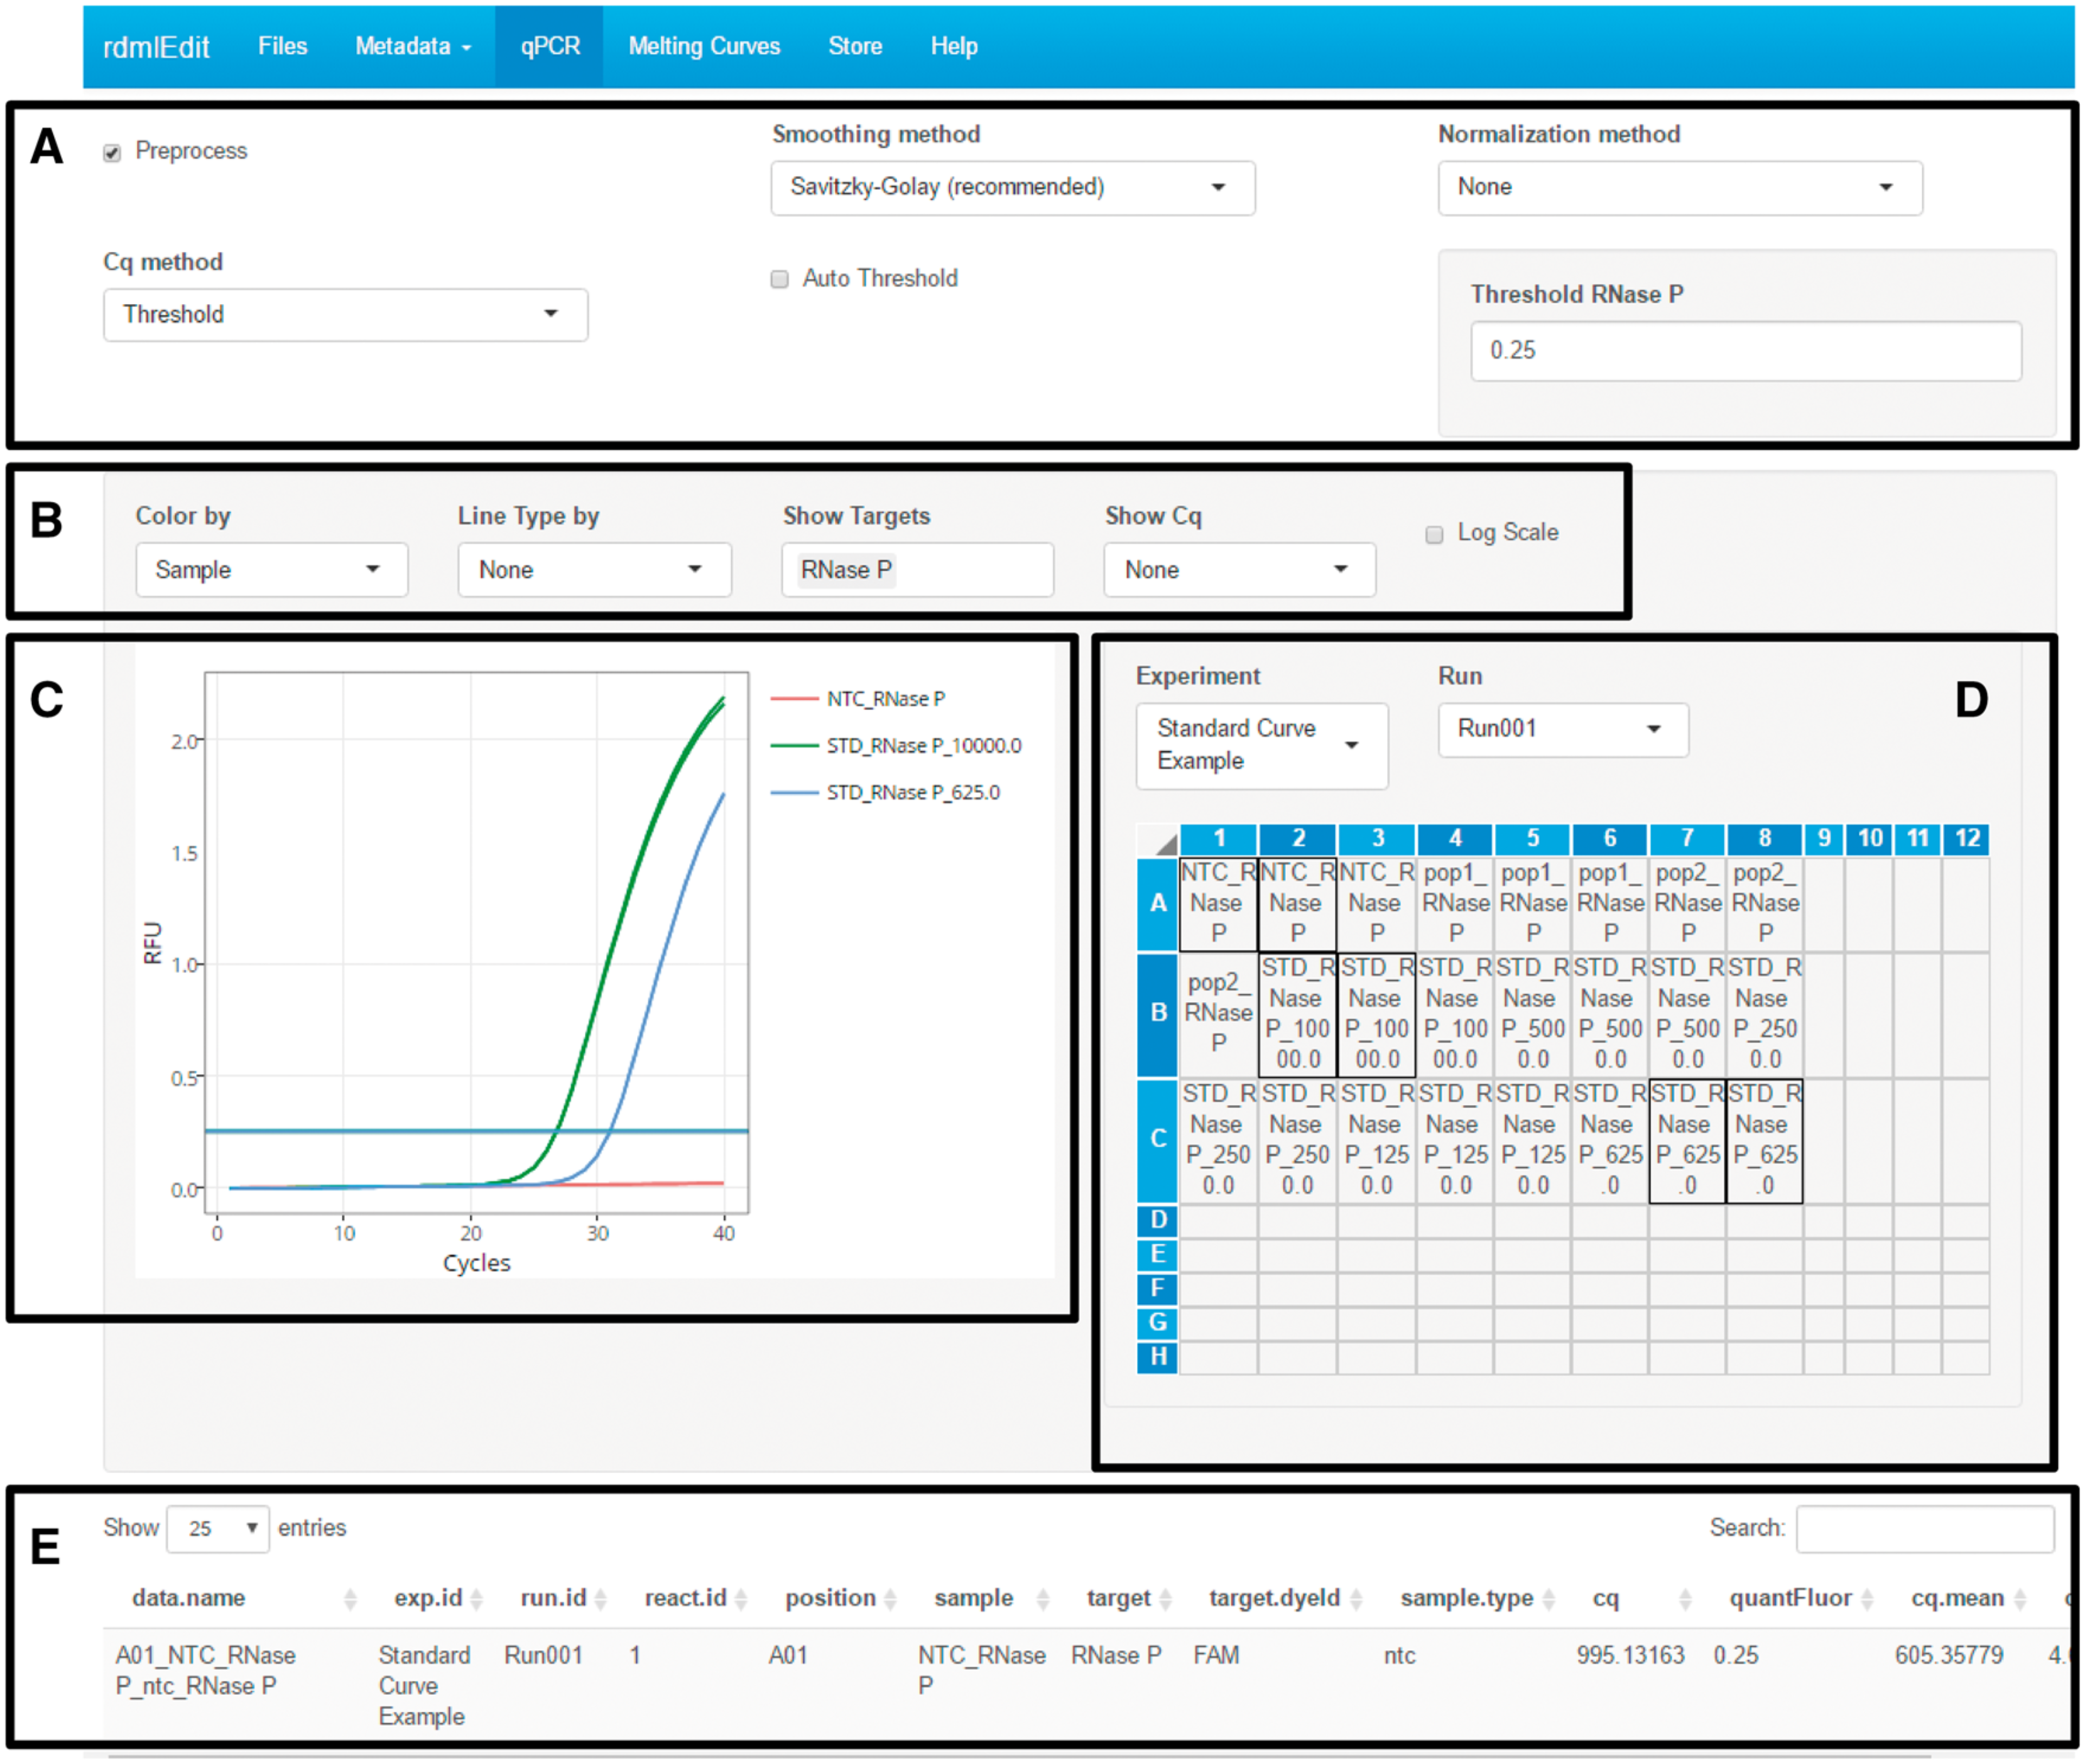
\includegraphics[width=0.75\textwidth]{static_figure/rdml.png}
\end{figure}

\tiny  R\"{o}diger S.,Burdukiewicz M., Spiess A.-N., Blagodatskikh 
K., Enabling reproducible real-time quantitative PCR research: the RDML 
package. 
Bioinformatics, 2017.

\end{frame}

\begin{frame}{chipPCR - walidacja urządzeń do PCR}
\begin{figure} 
\includegraphics[width=0.75\textwidth]{static_figure/chippcr.png}
\end{figure}

\tiny R\"{o}diger S., Burdukiewicz M., Schierack P., 
chipPCR: an R Package to Pre-Process Raw Data of Amplification Curves. 
Bioinformatics, 2015.

\end{frame}

\begin{frame}{Wpływ wygładzania danych na rezultaty eksperymentów PCR}
\begin{figure} 
\includegraphics[width=0.65\textwidth]{static_figure/smoothing.png}
\end{figure}

\tiny Spiess A.-N., Deutschmann C., Burdukiewicz M., Himmelreich 
R., 
Klat K., Schierack P., R\"{o}diger S., Impact of smoothing on parameter 
estimation in quantitative dna amplification experiments. Clinical 
Chemistry, 2014.

\end{frame}


\begin{frame}{Periodyczność rezultaty eksperymentów PCR}
\begin{figure} 
\includegraphics[width=0.65\textwidth]{static_figure/period.png}
\end{figure}

\tiny Spiess A.-N., R\"{o}diger S.,Burdukiewicz M., Volksdorf T., 
Tellinghuisen J., System-
specific periodicity in quantitative real-time polymerase chain reaction data 
questions
threshold-based quantitation, Scientific Reports, 2016.

\end{frame}


\begin{frame}{Podziękowania}
Mentorzy:
\begin{itemize}
\item \textbf{Paweł Mackiewicz (Uniwersytet Wrocławski)}.
\item Małgorzata Kotulska (Politechnika Wrocławska).
\item Marcin Łukaszewicz (Uniwersytet Wrocławski).
\item Andrzej Dąbrowski (Uniwersytet Wrocławski).
\item Stefan Rödiger (Brandenburg University of Technology Cottbus-Senftenberg).
\item Henrik Nielsen (Technical University of Denmark).
\item Lars Kaderali (University of Greifswald).
\item Andreas Weinhäusel (Austrian Institute of Technology).
\end{itemize}
\end{frame}


\begin{frame}{Podziękowania}
Współpracownicy:
\begin{itemize}
\item Przemysław Gagat (Uniwersytet Wrocławski).
\item Jarosław Chilimoniuk (Uniwersytet Wrocławski).
\item Rafał Kolenda (Uniwersytet Przyrodniczy we Wrocławiu).
\item Piotr Sobczyk (Politechnika Wrocławska).
\item Sławomir Jabłoński (Uniwersytet Wrocławski).
\item Marlena G\k{a}sior-Głogowska (Politechnika Wrocławska).
\item Chris Lauber (Technical University Dresden).
\item Anna Duda-Madej (Uniwersytet Medyczny im. Piastów Śląskich we Wrocławiu).
\end{itemize}

\end{frame}

\begin{frame}{Podziękowania}
Finansowanie:
\begin{itemize}
\item Narodowe Centrum Nauki (Preludium i Etiuda).
\item COST ACTION CA15110 (Harmonising standardisation strategies to increase efficiency and competitiveness of European life-science research).
\item KNOW Wrocław Center for Biotechnology.
\item InnoProfile-Transfer-Projekt 03IPT611X przyznanym przez Ministerstwo Edukacji i Badań Naukowych Niemiec.
\end{itemize}

\end{frame}

\begin{frame}[allowframebreaks]{Publikacje}

\small
\begin{enumerate}  

\item \underline{Burdukiewicz, M.}, Sobczyk, P., Chilimoniuk, J., Gagat, P., and Mackiewicz, P., \textit{Prediction of Signal Peptides in Proteins from Malaria Parasites}. \textbf{International Journal of Molecular Sciences}, 2018.

\item Kolenda R., \underline{Burdukiewicz M.}, Schiebel J., Rödiger S, Sauer L., Szabo I., Orłowska A., Weinreich J., Nitschke J., Böhm, A., Gerber U., Roggenbuck D., Schierack P., \textit{Adhesion of Salmonella to pancreatic secretory granule membrane major glycoprotein GP2 of human and porcine origin depends on FimH sequence variation}, \textbf{Frontiers in microbiology}, 2018.

\item Mackiewicz D., Posacki P., \underline{Burdukiewicz M.}, Błażej P. \textit{Role of recombination and faithfulness to partner in sex chromosome degeneration}. \textbf{Scientific Reports}, 2018.

\item \underline{Burdukiewicz M.}, Gagat P. Jab\l{}o\'nski S., Chilimoniuk J., 
Gaworski M., Mackiewicz P., \L{}ukaszewicz M. \textit{PhyMet2: a database and toolkit for phylogenetic and metabolic analyses of methanogens}.
\textbf{Environmental Microbiology Reports}, 2018.

\item \underline{Burdukiewicz M.}, Sobczyk P. R\"{o}diger S., Duda-Madej A., 
Mackiewicz P., Kotulska M., \textit{Amyloidogenic motifs revealed by n-gram 
analysis}. 
\textbf{Scientific Reports}, 2017. 

\item Schiebel J., B\"{o}hm A., Nitschke J., \underline{Burdukiewicz M.}, 
Weinreich J., Ali A., Roggenbuck
D., R\"{o}diger S., Schierack P., \textit{Genotypic and phenotypic 
characteristics in association
with biofilm formation in different pathotypes of human clinical Escherichia 
coli isolates},
\textbf{Applied and Environmental Microbiology}, 2017.

\item R\"{o}diger S., \underline{Burdukiewicz M.}, Spiess A.-N., Blagodatskikh 
K., \textit{Enabling reproducible real-time quantitative PCR research: the RDML 
package}. 
\textbf{Bioinformatics}, 2017.

\item \underline{Burdukiewicz M.}, R\"{o}diger S., Sobczyk P., Menschikowski 
M., Schierack P.,
Mackiewicz P., \textit{Methods for comparing multiple digital PCR experiments}, 
\textbf{Biomolecular
Detection and Quantification}, 2016.

\item Spiess A.-N., R\"{o}diger S., \underline{Burdukiewicz M.}, Volksdorf T., 
Tellinghuisen J., \textit{System-
specific periodicity in quantitative real-time polymerase chain reaction data 
questions
threshold-based quantitation}, \textbf{Scientific Reports}, 2016.

\item Kolenda R., \underline{Burdukiewicz M.}, Schierack P., \textit{A 
systematic review and meta-analysis of the epidemiology of pathogenic 
escherichia coli of calves and the role of calves as reservoirs for human 
pathogenic E. coli}. \textbf{Frontiers in Cellular and Infection Microbiology}, 
2015.

\item R\"{o}diger S., \underline{Burdukiewicz M.}, Schierack P., 
\textit{chipPCR: an R Package to Pre-Process Raw Data of Amplification Curves}. 
\textbf{Bioinformatics}, 2015.

\item R\"{o}diger S., \underline{Burdukiewicz M.}, Blagodatskikh K., Jahn M., 
Schierack P., 
\textit{R as an
Environment for the Reproducible Analysis of DNA Amplification Experiments}, 
\textbf{R Journal}, 2015.

\item Spiess A.-N., Deutschmann C., \underline{Burdukiewicz M.}, Himmelreich 
R., 
Klat K., Schierack P., R\"{o}diger S., \textit{Impact of smoothing on parameter 
estimation in quantitative dna amplification experiments}. \textbf{Clinical 
Chemistry}, 2014.

\end{enumerate}
\end{frame}


\begin{frame}[allowframebreaks]
        \frametitle{References}
  \bibliographystyle{apalike}
  \bibliography{references}
\end{frame}  


\end{document}
